\documentclass{beamer}
\usepackage[utf8]{inputenc}
\usepackage{listings}
\usepackage{booktabs}
\usepackage{amssymb}
\usepackage{nicefrac}
\usepackage{amsmath}
\usepackage{bbm}
\usepackage{bm}
\usepackage{enumitem}
\usepackage{hyperref}
\usepackage[export]{adjustbox}
\usepackage{animate}
\usepackage{svg}

\usetheme{Madrid}
\definecolor{mlpblue}{rgb}{0.1, 0.14, 0.24}

\useoutertheme{infolines} % Alternatively: miniframes, infolines, split
\useinnertheme{circles}
\usecolortheme[named=mlpblue]{structure}

\DeclareMathOperator{\Tr}{Tr}
\DeclareMathOperator{\Cov}{Cov}
\DeclareMathOperator{\Concat}{Concat}

\DeclareMathOperator*{\argmax}{arg\,max}
\DeclareMathOperator*{\argmin}{arg\,min}
\DeclareMathOperator*{\indep}{\perp \!\!\! \perp}

\lstset{basicstyle=\footnotesize\ttfamily,breaklines=true}

%------------------------------------------------------------
%This block of code defines the information to appear in the
%Title page
\title[Active Vision for Bi-Manipulator Systems]{Perception Aware Planning}

%\subtitle{Extending Mpinets} %\thanks{Beaglehole, Súkeník et.~al.~[NeurIPS 2024]}}


\author[CS 592-RM]{A. Buynitsky} 

\date{Dec 10, 2024}

\titlegraphic{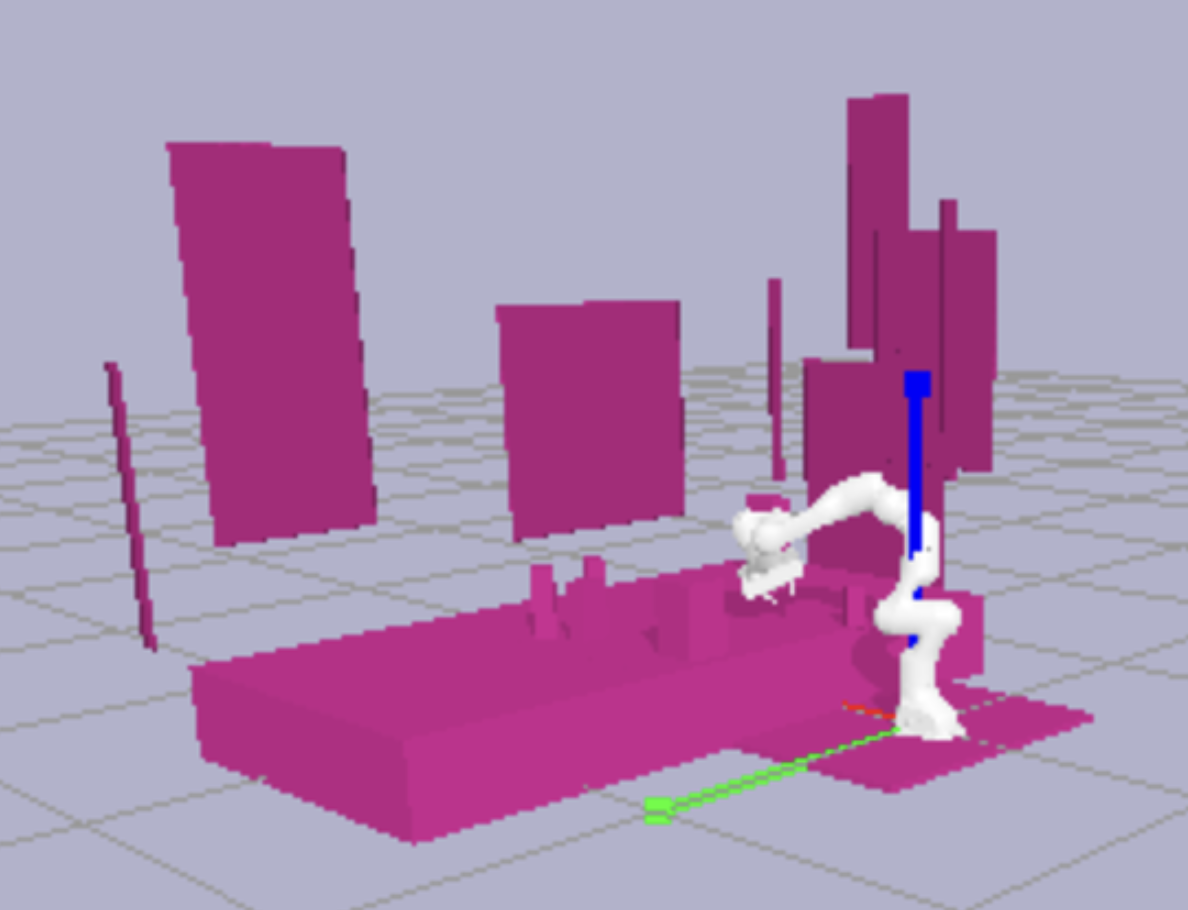
\includegraphics[width=5cm]{./img/title_page.png}}

%End of title page configuration block
%------------------------------------------------------------

%The next block of commands puts the table of contents at the 
%beginning of each section and highlights the current section:

\AtBeginSection[]
{
  \begin{frame}
    \frametitle{Outline}
    \tableofcontents[currentsection]
  \end{frame}
}
% ------------------------------------------------------------


\begin{document}

\frame{\titlepage}


%---------------------------------------------------------
% This block of code is for the table of contents after
% the title page
\begin{frame}
\frametitle{Outline}
\tableofcontents
\end{frame}
%---------------------------------------------------------
\section{Motivation}
\begin{frame}[t]{Manipulate-Anything}
    \vspace{-1em}
    Many approaches use either a fixed viewpoint or a collection of viewpoints.
    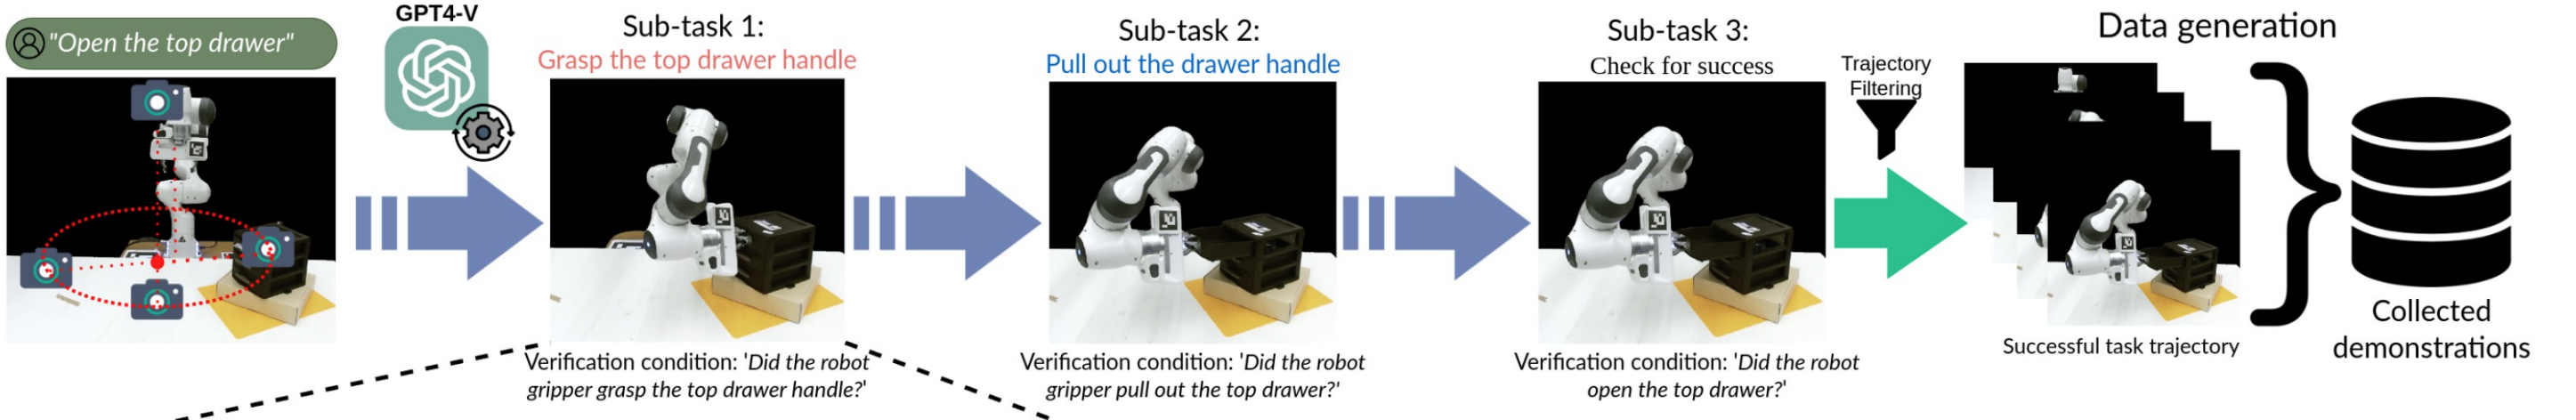
\includegraphics[width=\textwidth]{./img/motivation_0.png}
    \textbf{Approach:} Decomposes a task into smaller subtasks with VLM
    %\textbf{Uses 4 RGB-d cameras positioned around the table}
    \pause
    \begin{columns}
		\begin{column}{.5\textwidth}
            \begin{center}
                \vspace{-1em}
                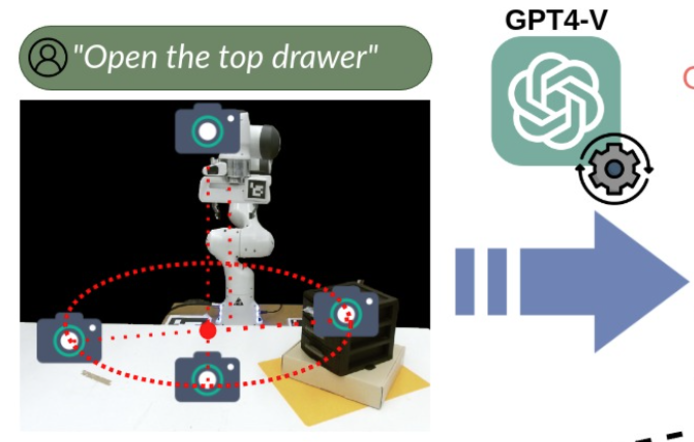
\includegraphics[width=\textwidth]{./img/motivation_1.png}
            \end{center}
		\end{column}
		\hspace{1em}
		\begin{column}{.5\textwidth}
            \textbf{Problem:} Uses 4 RGB-D cameras placed around the scene. Then Select a viewpoint or a combination of viewpoints for each subtask.
		\end{column}
	\end{columns}
\end{frame}

\begin{frame}[t]{Perceiver-Actor}
    \vspace{-1em}
    Many approaches use either a fixed viewpoint or a collection of viewpoints.
    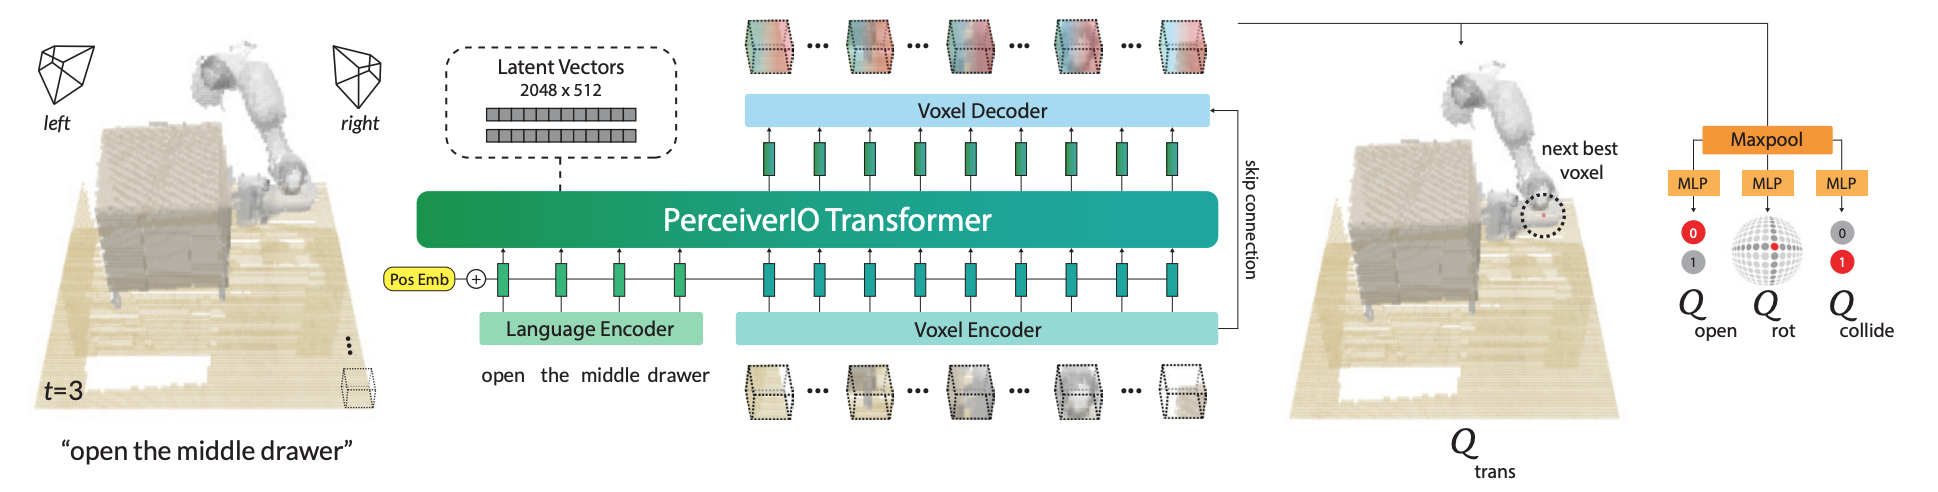
\includegraphics[width=\textwidth]{./img/motivation_peract_0.png}
    \textbf{Approach:} Takes language goal and RGB-D voxel as input, predicts discrete actions 
    %\textbf{Uses 4 RGB-d cameras positioned around the table}
    \pause
    \begin{columns}
		\begin{column}{.5\textwidth}
            \begin{center}
                \vspace{-1em}
                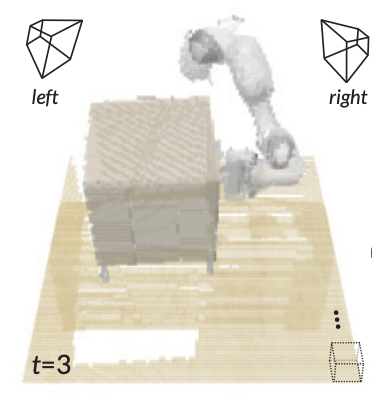
\includegraphics[width=0.5\textwidth]{./img/motivation_peract_1.png}
            \end{center}
		\end{column}
		\hspace{1em}
		\begin{column}{.5\textwidth}
            \textbf{Problem:} Uses 4 RGB-D cameras to construct an occlusion-free voxel representation of the scene.
		\end{column}
	\end{columns}
\end{frame}

\begin{frame}[t]{Problem: Manipulation under Occlusion}
    The majority of approaches assume either:
    \begin{itemize}[label=-]
        \item an occlusion-free view from a fixed camera
        \item the ability to construct an occlusion-free representation of a scene from multiple viewpoints 
    \end{itemize}
    Most motion planners would fail to generate successful trajectories in occluded, crowded environments 
    \pause
    \newline
    \textbf{Project Goal:} Active Vision / Sensing in bi-manupulator systems 
    \begin{center}
    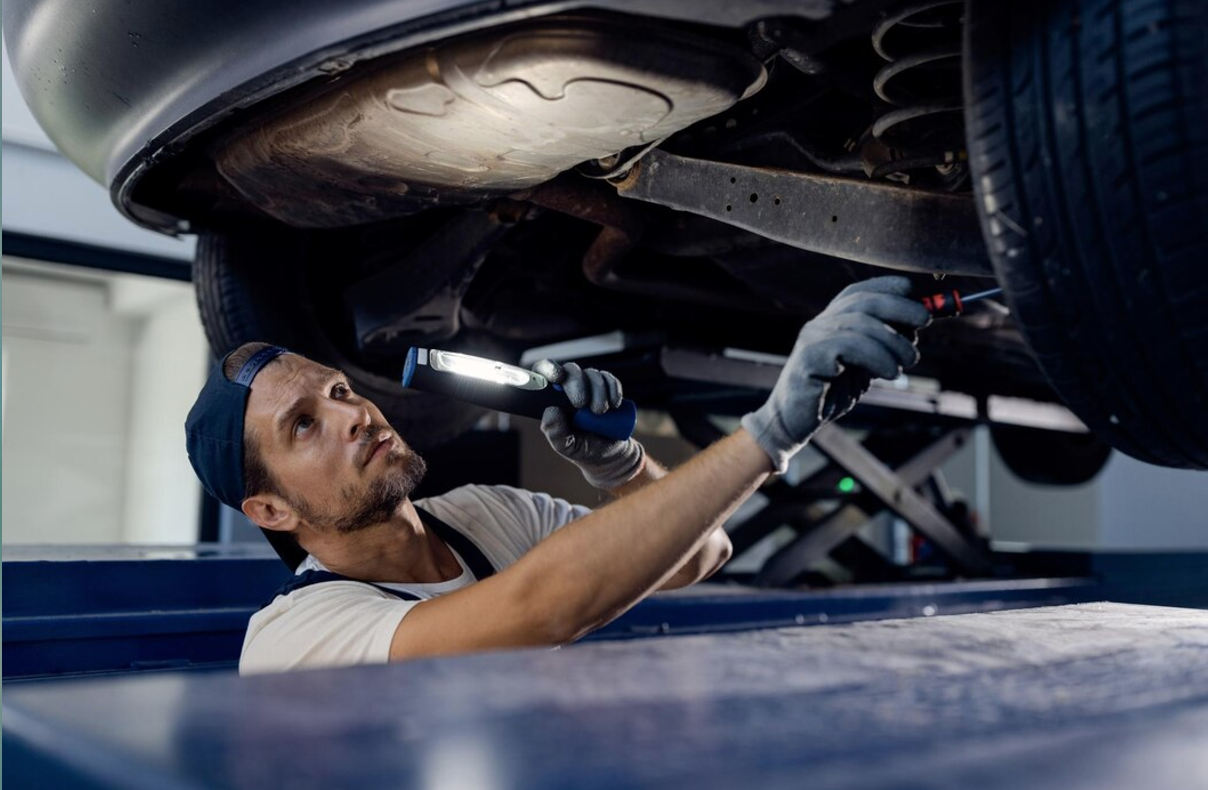
\includegraphics[width=0.5\textwidth]{./img/motivation_2.png}
    \end{center}

    
\end{frame}



\section{Related Work}
\begin{frame}[t]{Observe Then Act}
    \small
    Use a dual-agent structure consisting of two policies: 
    \begin{itemize}
        \item \textbf{Next-Best-View (NBV)}: infer optimal viewpoints 
        \item \textbf{Next-Best-Pose (NBP)}: predict next discrete 6-DOF gripper pose 
    \end{itemize}
    \pause
    Formulate as POMDP, dividing one interaction into a NBV action and NBP action
    \begin{center}
    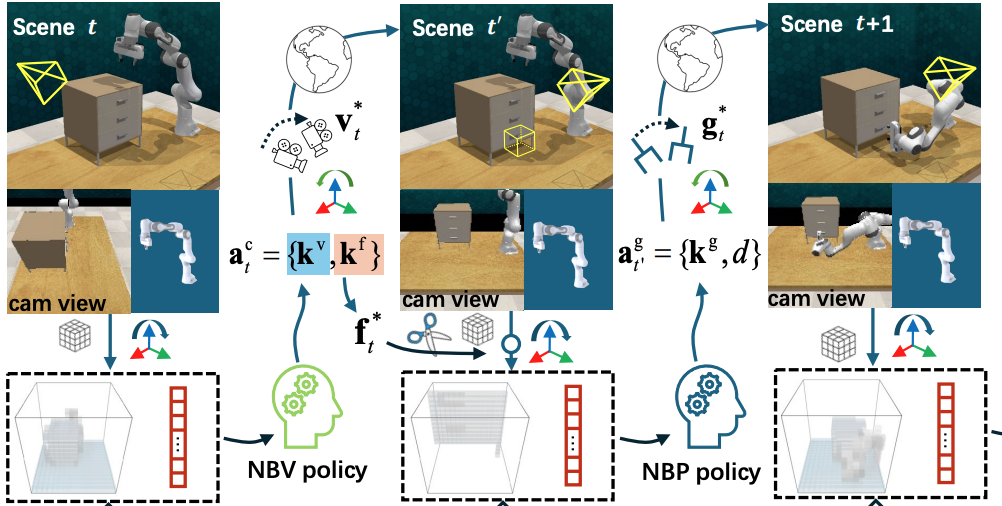
\includegraphics[width=0.55\textwidth]{./img/observe_then_act_0.png}
    \end{center}
    \textbf{Reward:} Sum of whether the training episode was completed, (reached ROI), reduction of entropy in voxel occupancy, and reachible ROI.
    \pause
    \newline
    \textbf{Limitation:} Camera position is limited to the upper half-plane at a fixed radius
\end{frame}

\begin{frame}[t]{3D Move To See}
    \small
    Solve for gradient of the objective function representing the goal of the system
    \newline
    \textbf{Objective Function} consists of two parts:
    \begin{itemize}[label=-]
        \item occlusion of the target object
        \item robot manipulability score
    \end{itemize}
    \begin{columns}
		\begin{column}{.5\textwidth}
            \begin{center}
                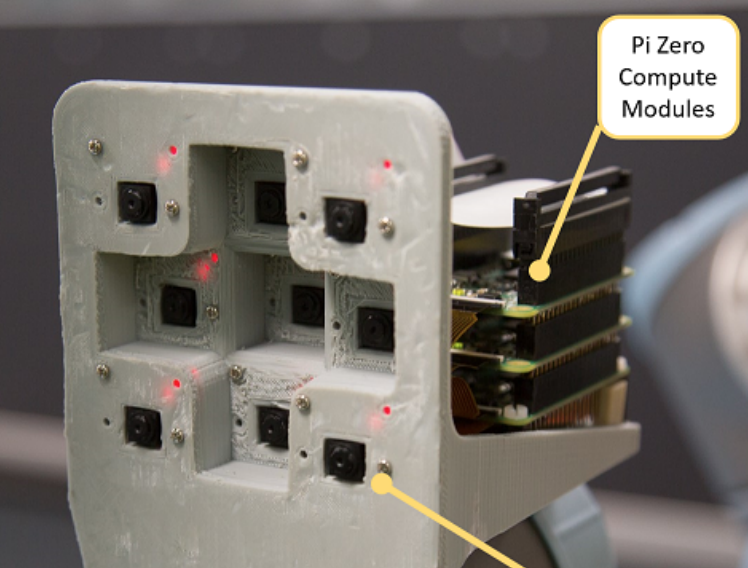
\includegraphics[width=0.8\textwidth]{./img/3d_move_to_see_0.png}
            \end{center}
		\end{column}
		\hspace{1em}
		\begin{column}{.5\textwidth}
                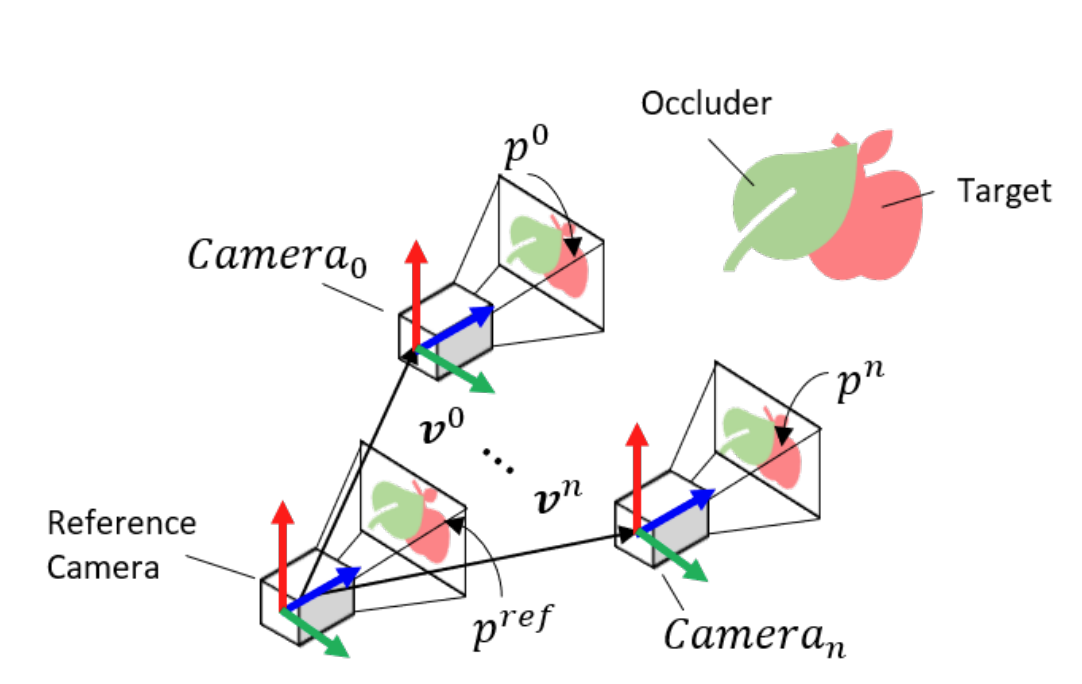
\includegraphics[width=1.\textwidth]{./img/3d_move_to_see_1.png}
		\end{column}
	\end{columns}
    \vspace{1em}


    \textbf{Limitation:}  Camera can get caught in a local minimum
\end{frame}

\begin{frame}[t]{Active Sensing and Planning in Cluttered Envs}
    \small
    \textbf{Goal:} maximize scene convergence in the least time steps
         \[
        \max_{v^t \sim \pi} \min_T \sum_{t=0}^{T-1} \phi(S_o^{t+1}(v^t) \setminus S_o^t, S)
        \]
    \newline
    \textbf{Score Net:} NN approach forecast scene convergence at various viewpoints 
    \newline
    \textbf{Trajectory Generation:} Generate the next viewpoint that maximizes scorenet score via MPC or transformer
    \begin{center}
        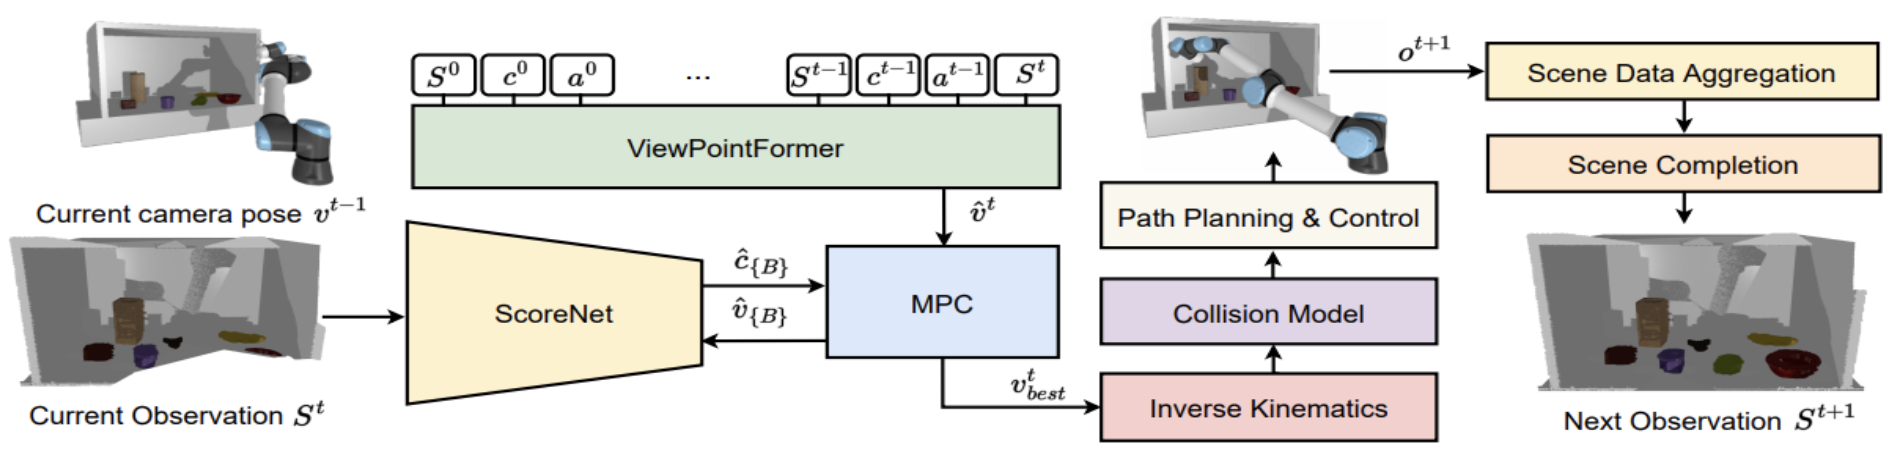
\includegraphics[width=0.8\textwidth]{./img/action_sensing_0.png}
    \end{center}
    \vspace{1em}


    \textbf{Limitation:} Single manipulator exploring an unknown environment 
\end{frame}


\begin{frame}[t]{ACT + AV-Aloha}
    \small
    \textbf{Robotic System:} 3 total robotic arms (2 manipulators + one camera)
    \begin{center}
    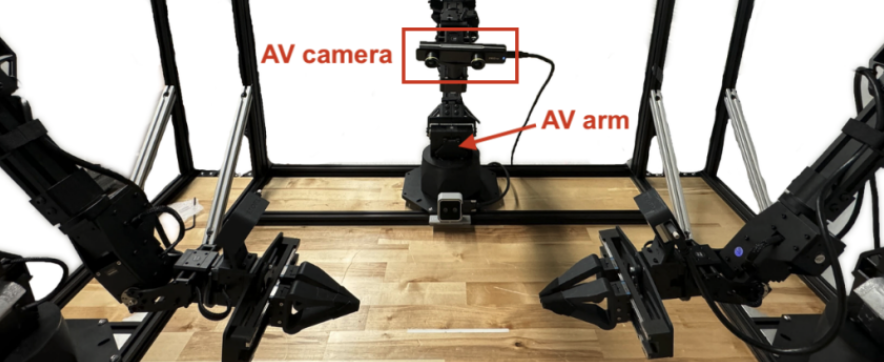
\includegraphics[width=0.4\textwidth]{./img/av_aloha_0.png}
    \end{center}
    \pause
    \textbf{Data Generation:} Data for manipulator arms collected from human grippers
    \begin{itemize}[label=-]
      \item Data for manipulator arms collected from human grippers
      \item Data for AV arm collected from Oculus headset
    \end{itemize}
    \pause
    \textbf{Training:} Train with ACT (Action-Chunking Transformer) - predict the next 50 actions at each time step via Imitation Learning
    \begin{center}
    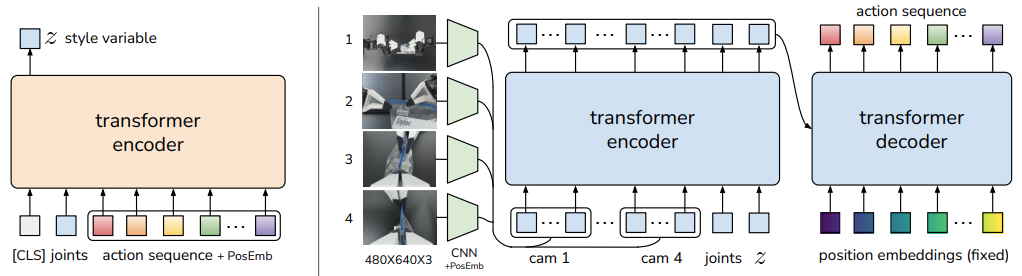
\includegraphics[width=0.7\textwidth]{./img/av_aloha_1.png}
    \end{center}
\end{frame}


\section{Baseline}
\begin{frame}[t]{M$\pi$nets}
    Generate collision-free smooth motion plans from a single-depth camera observation.
    \\
    \textbf{Training:} Trained on 3 million trajectories in 500,000 environments with behavioral cloning to predict c-space waypoints.
    \\
    \textbf{Architecture:}
    \begin{center}
        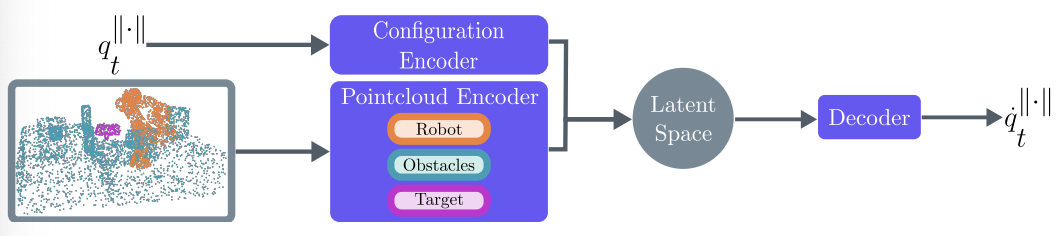
\includegraphics[width=1.\textwidth]{./img/mpinet_0.png}
    \end{center}
\end{frame}

\section{Extending Baseline}
\begin{frame}[t]{Reproducing Results}
    Faced problems with setting up the repo (dell xps + vm failed)
    and CoRAL server lost power multiple times...
    \begin{center}
        \only<1>{
        \begin{center}
            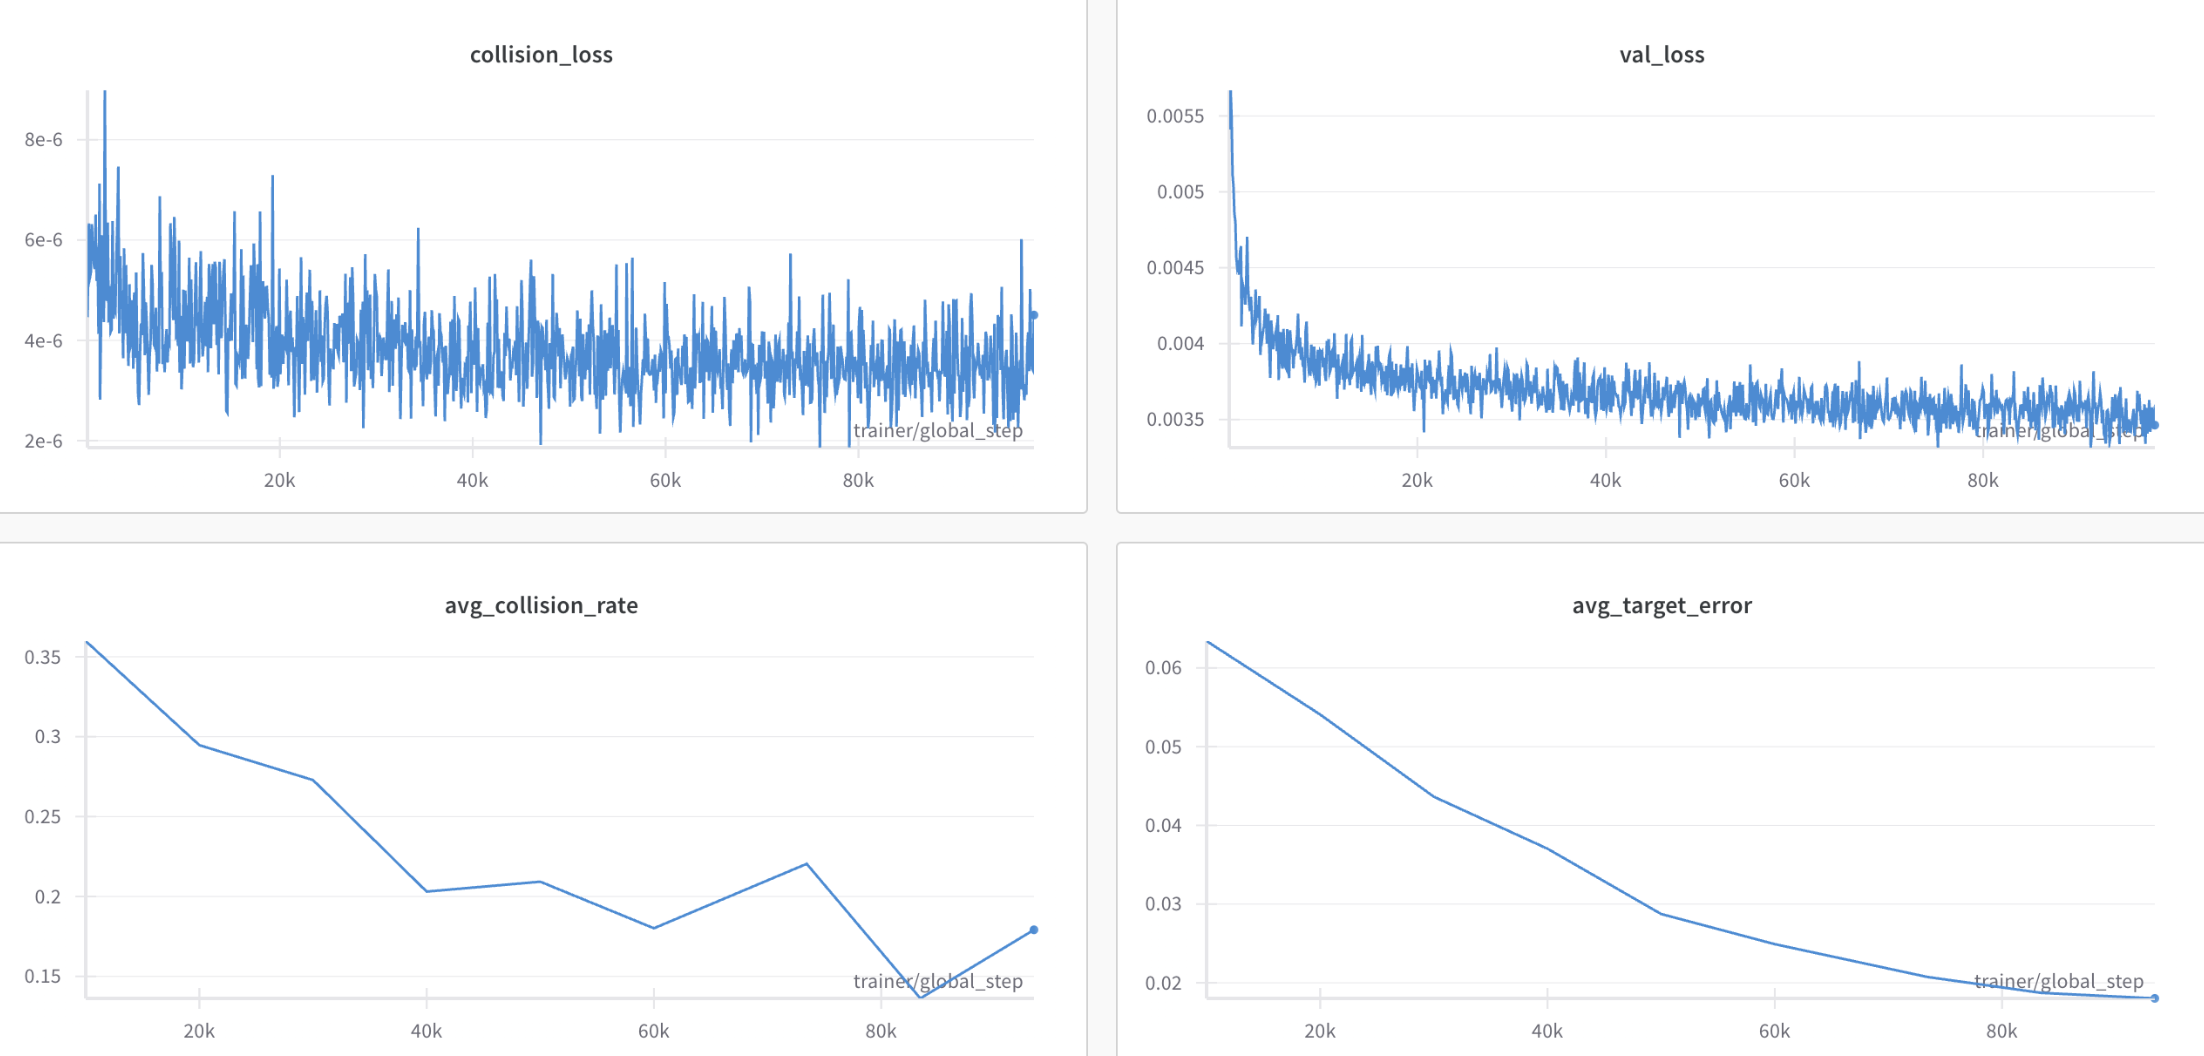
\includegraphics[width=0.9\textwidth]{./img/reproducing_0.png}
        \end{center}
        }
        \only<2>{
        \begin{center}
            \animategraphics[loop,width=0.9\textwidth]{10}{./img/mpinet_gif/mpinet_demo-}{0}{23}
        \end{center}
        }
    \end{center}
\end{frame}


\begin{frame}[t]{Creating Custom dataset (Part 1)}
    M$\pi$nets input consists of 3 point clouds: obstacles, target location, robot point cloud
    \\
    A dataset with occlusions will project the obstacle pointcloud on some camera locations.
    \\
    \textbf{Dataset Samples:}
    \begin{columns}
		\begin{column}{.4\textwidth}
            \begin{center}
                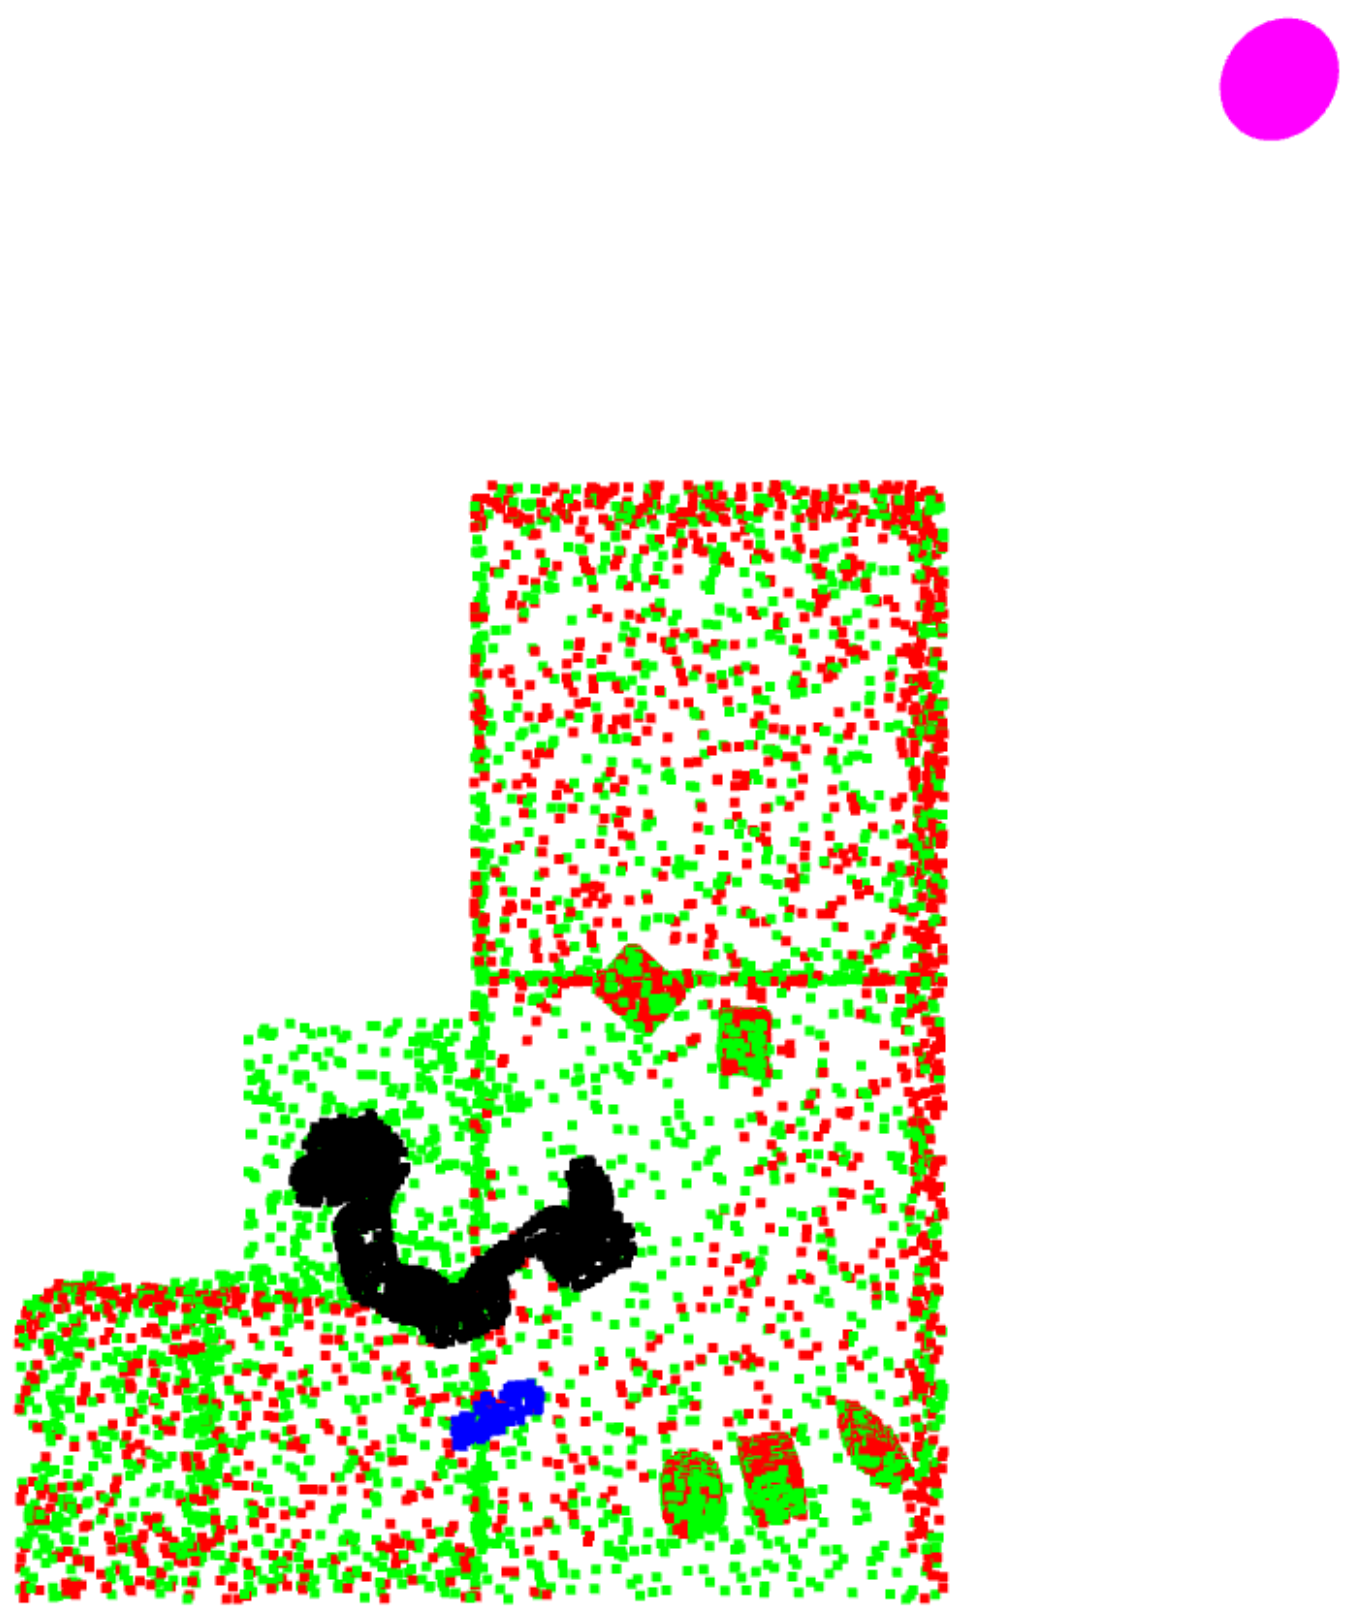
\includegraphics[width=0.8\textwidth]{./img/ds_0.png}
            \end{center}
		\end{column}
		\begin{column}{.4\textwidth}
                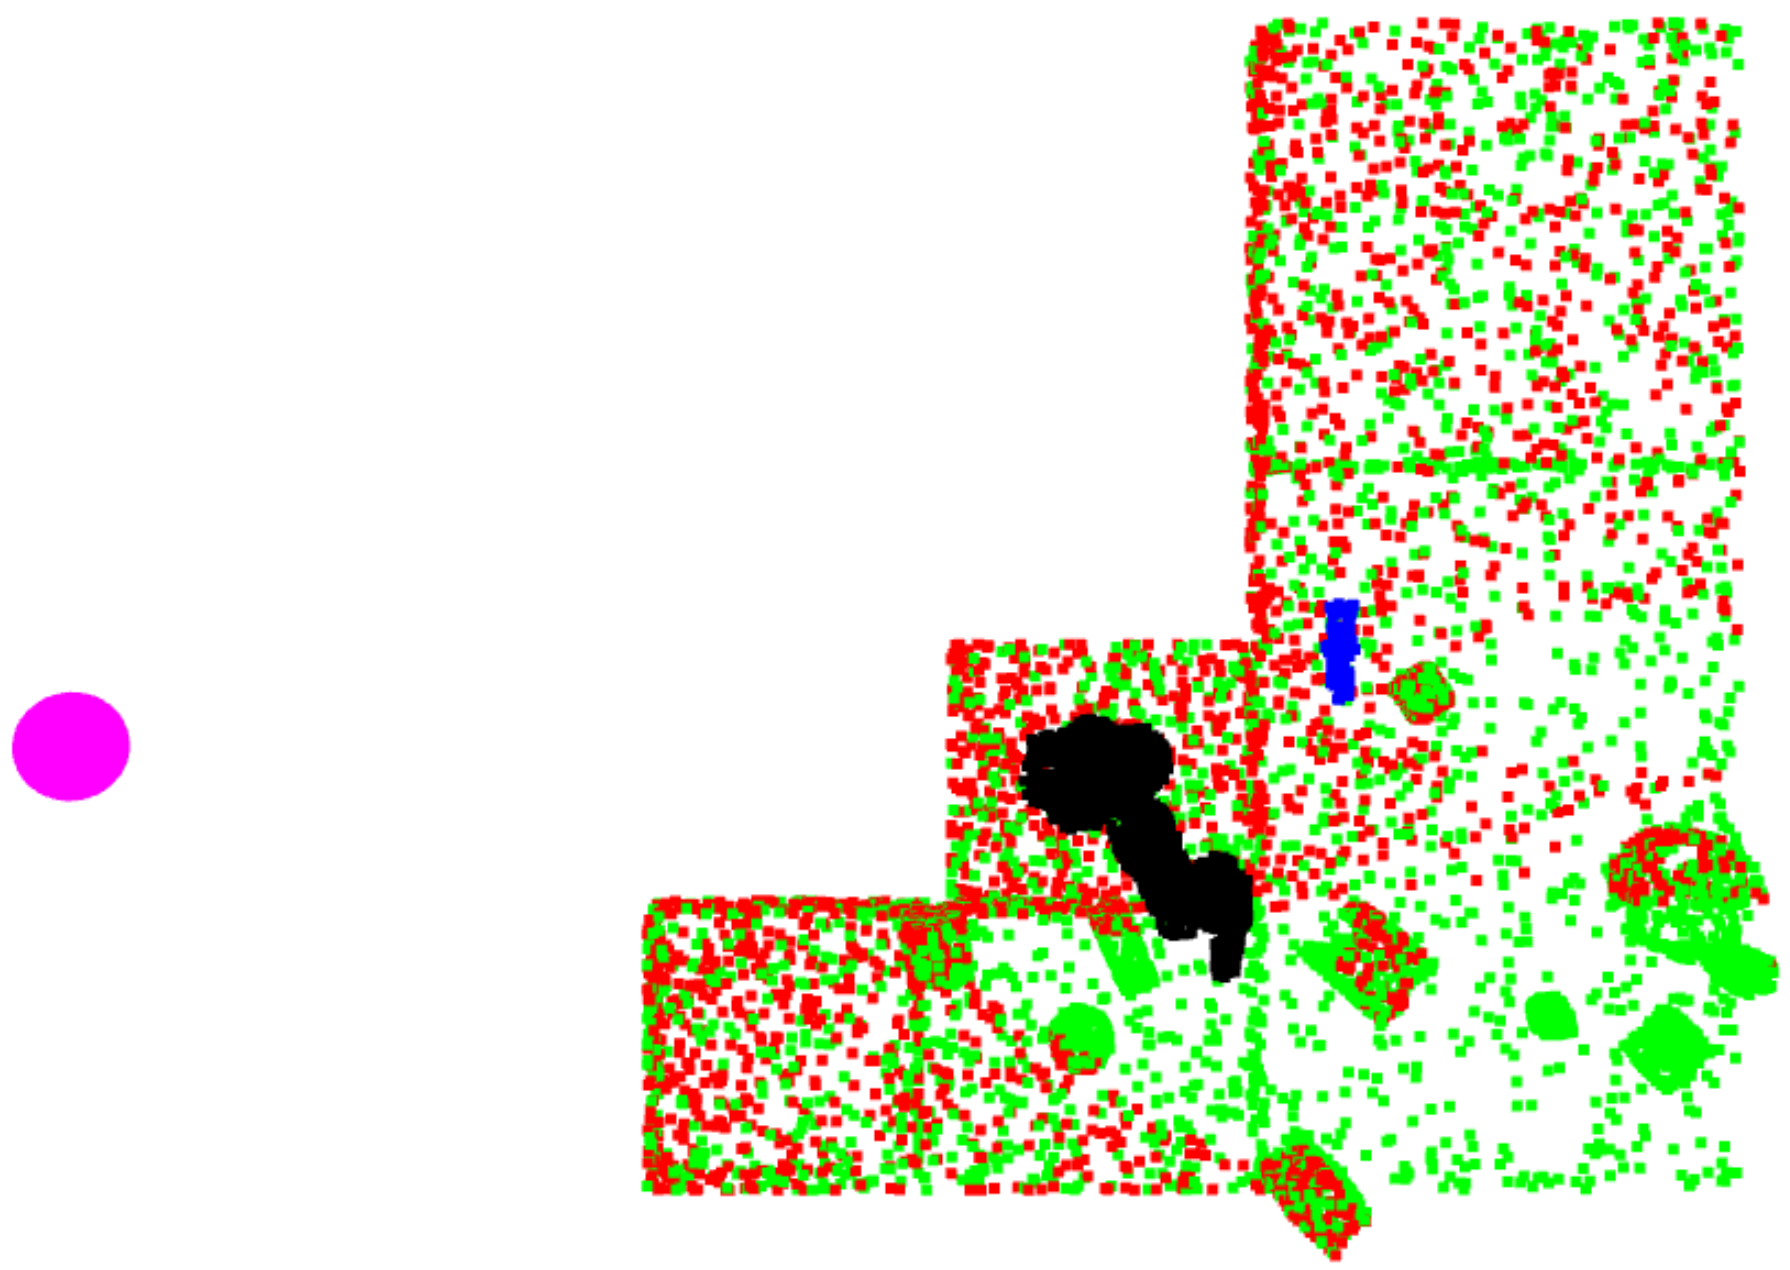
\includegraphics[width=1.\textwidth]{./img/ds_1.png}
		\end{column}
		\begin{column}{.3\textwidth}
                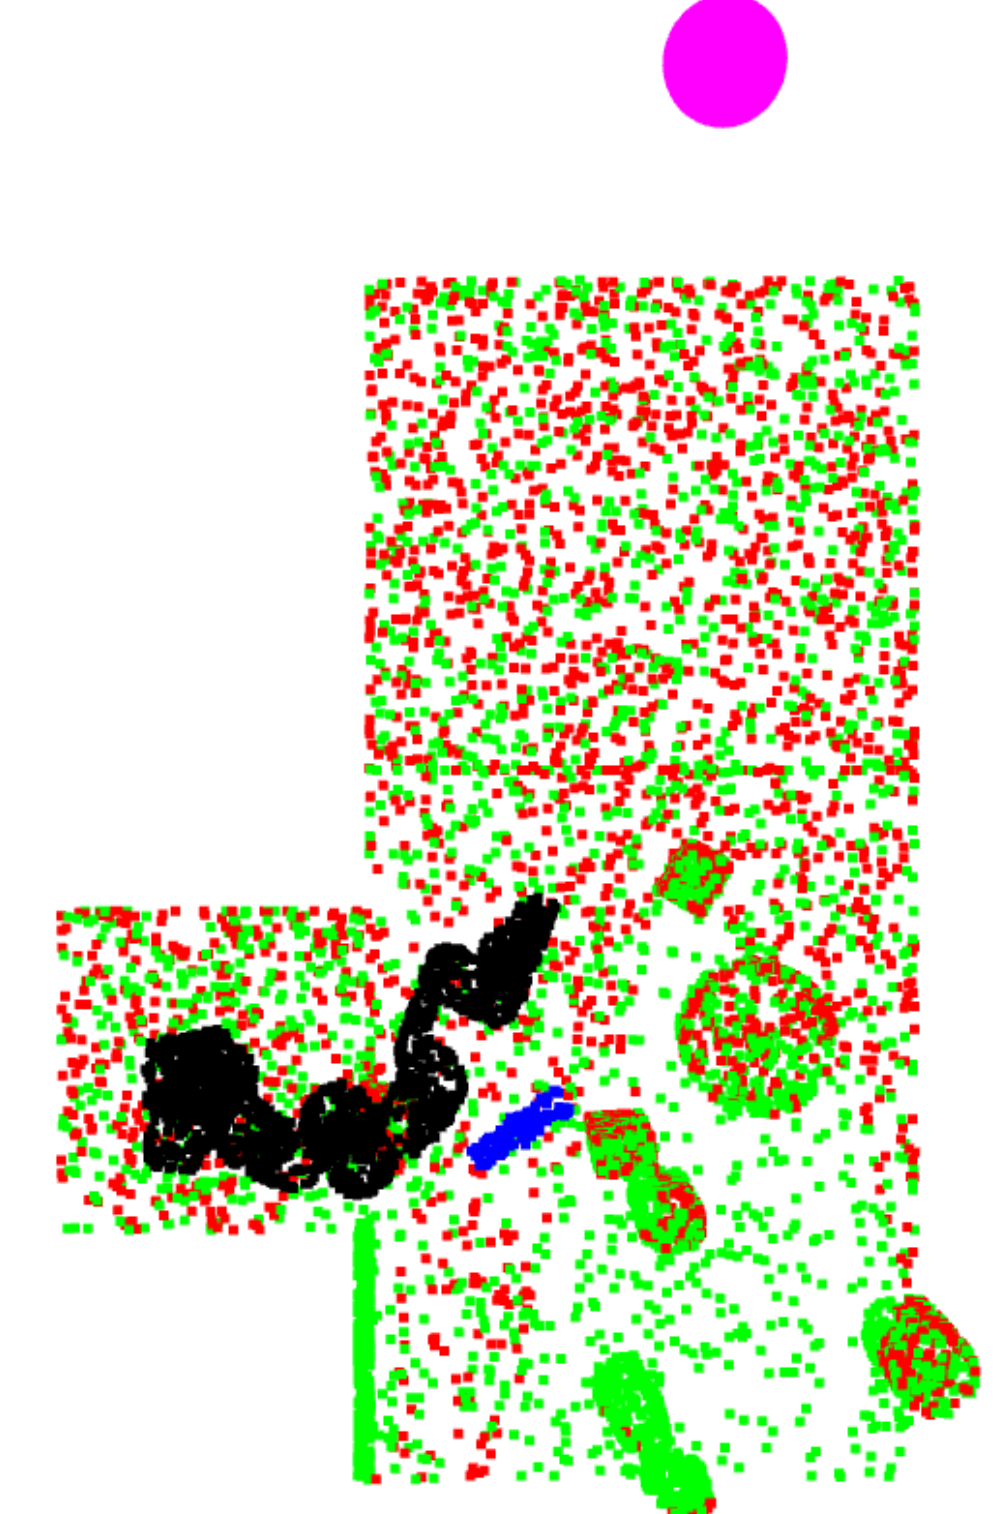
\includegraphics[width=0.7\textwidth]{./img/ds_2.png}
		\end{column}
	\end{columns}
\end{frame}

\begin{frame}[t]{Creating Custom dataset (Part 2)}
    Generated sensible occlusions around the perimeter  of the robot's workspace and within it:
    \\
    \textbf{Dataset Samples:}
    \\
    \begin{columns}
		\begin{column}{.5\textwidth}
        \begin{center}
            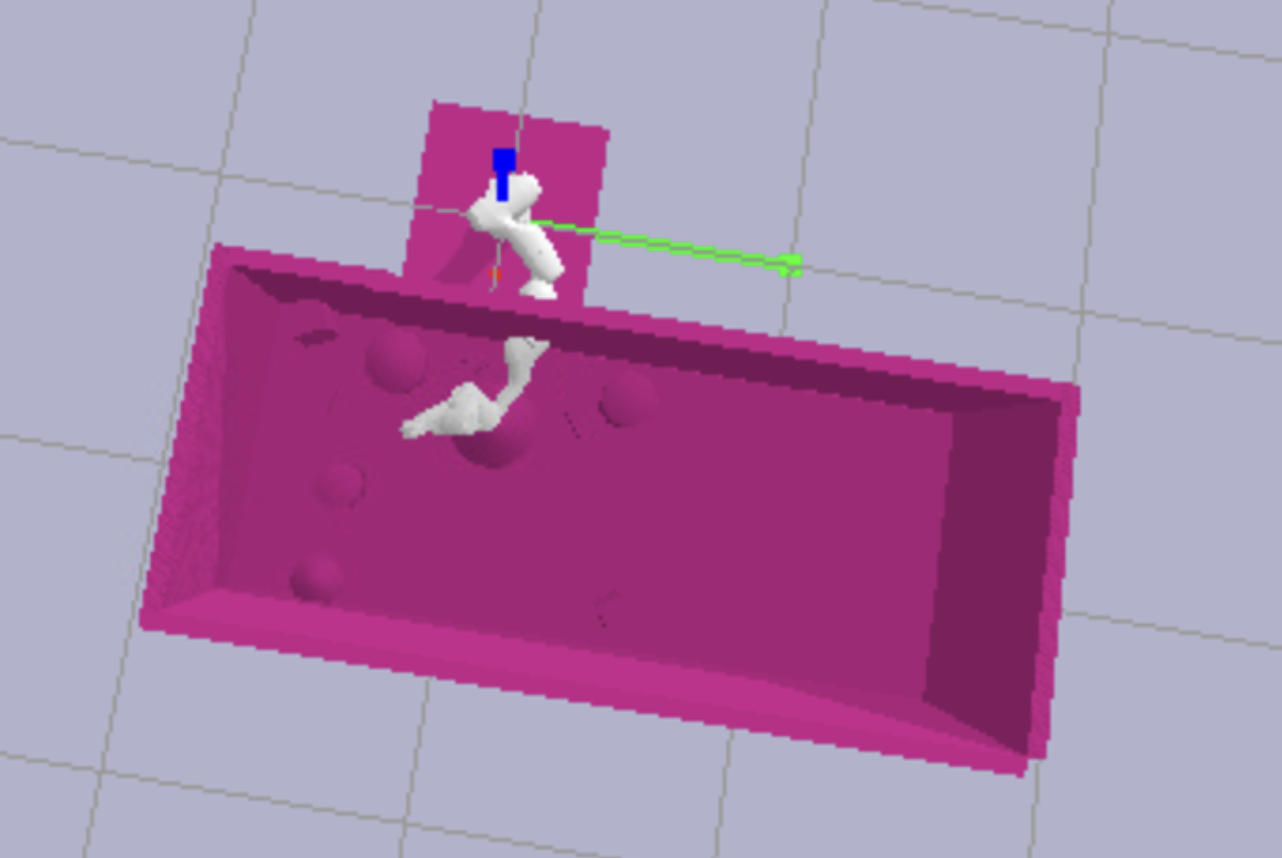
\includegraphics[width=0.8\textwidth]{./img/ds_2_0.png}
        \end{center}
		\end{column}
		\begin{column}{.5\textwidth}
            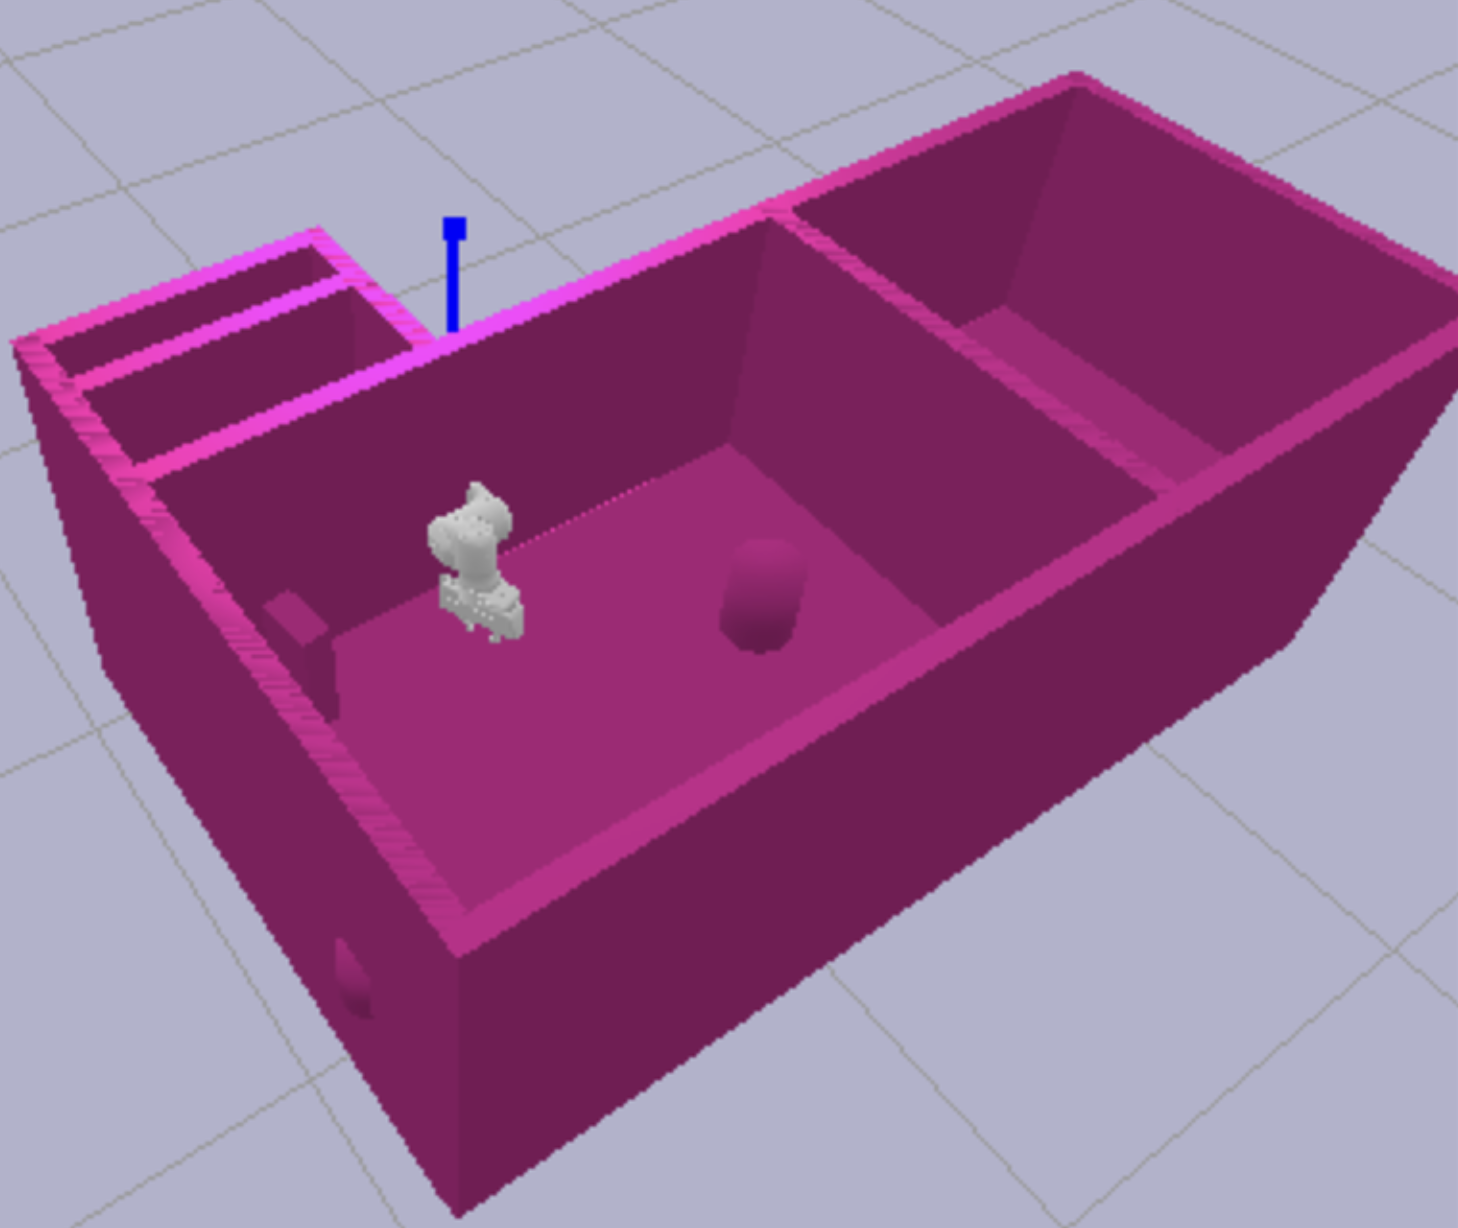
\includegraphics[width=0.8\textwidth]{./img/ds_2_1.png}
		\end{column}
	\end{columns}
\end{frame}

\begin{frame}[t]{Creating Custom dataset (Part 3)}
    Generate occlusions around perimeters/borders, representing obstacles (i.e. a human leaning over)
    \\
    \textbf{Dataset Samples:}
    \\
    \begin{center}
        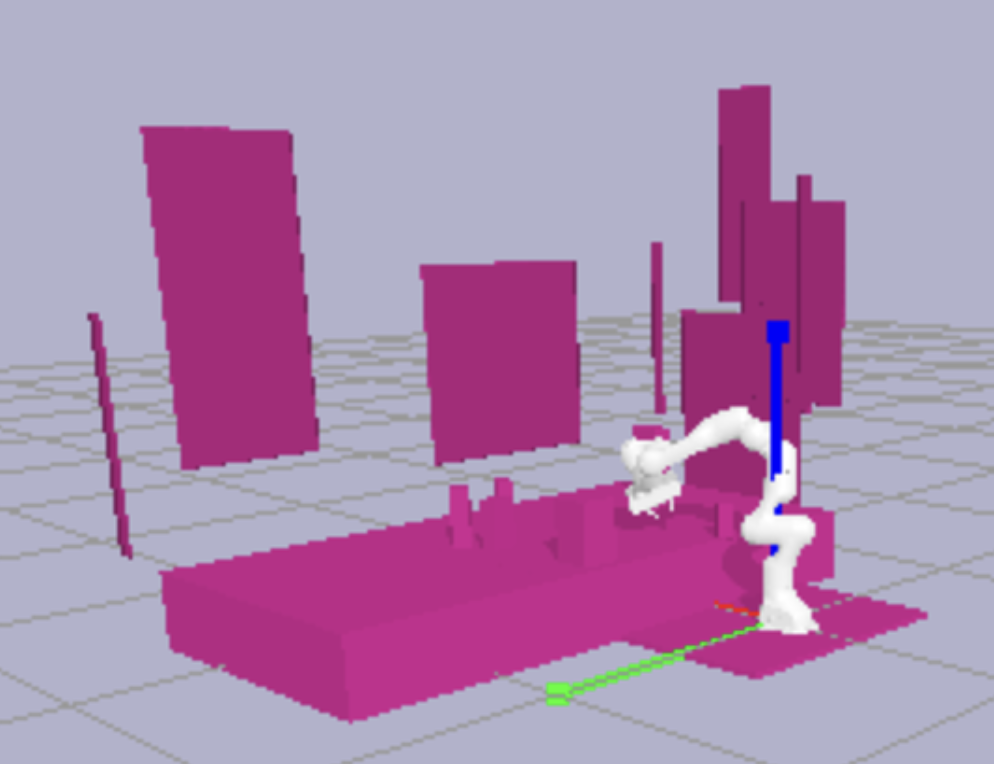
\includegraphics[width=0.6\textwidth]{./img/ds_3_0.png}
    \end{center}
\end{frame}


\begin{frame}[t]{Training Comparison}
    Receive identical training curves with occlusion vs no occlusions
    \begin{center}
        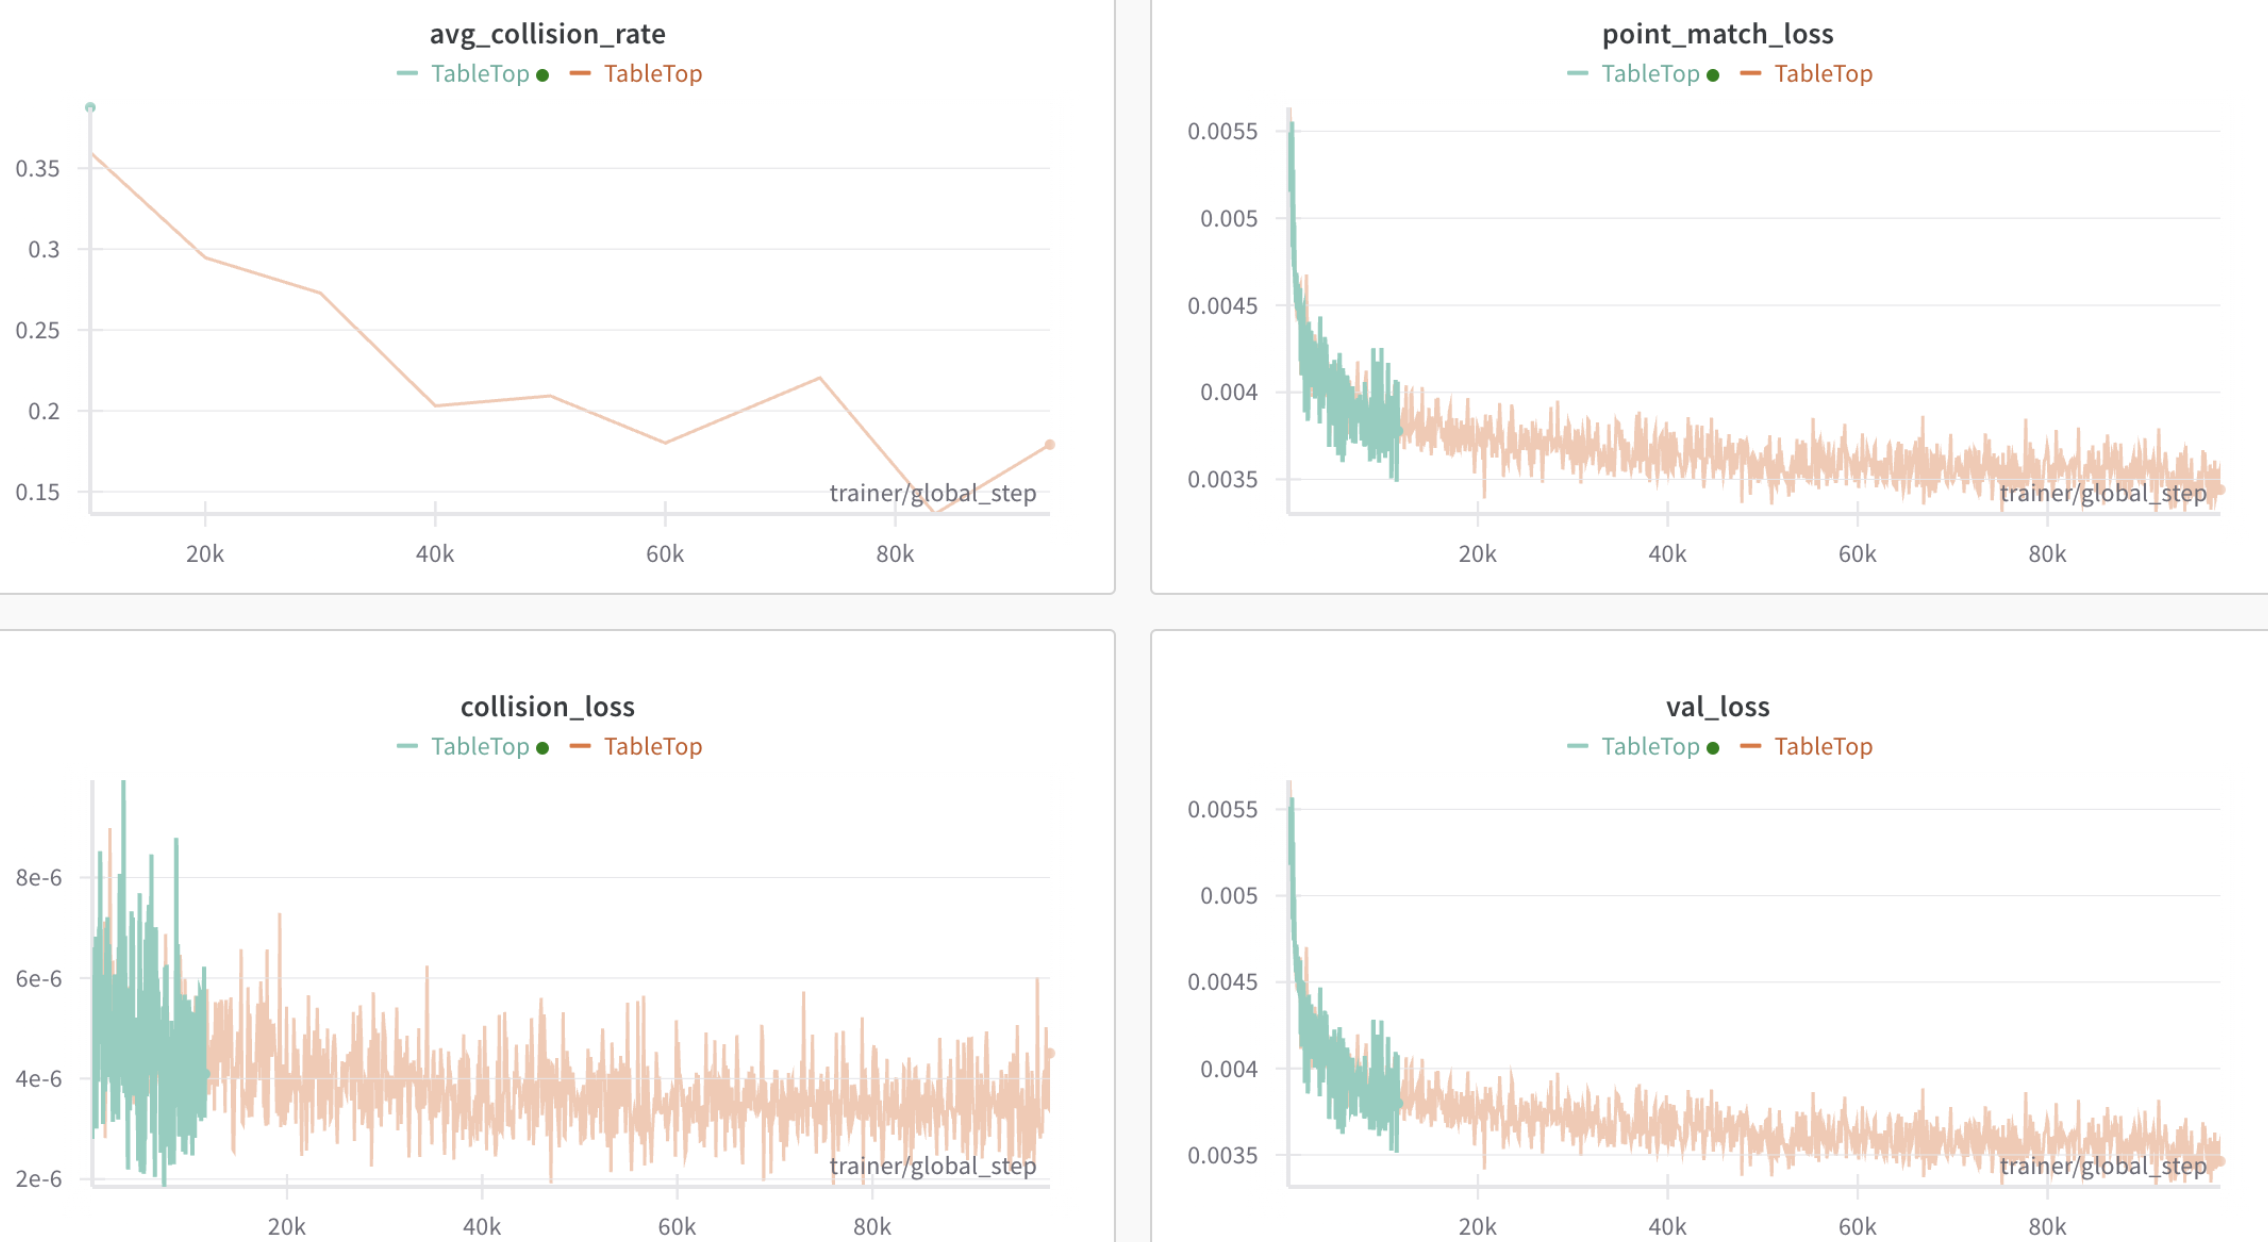
\includegraphics[width=0.6\textwidth]{./img/train_cmp_0.png}
    \end{center}
    \pause
    \textbf{Problem:} Collision loss computes the pointcloud with occlusions
\end{frame}

\section{Future Work}
\begin{frame}[t]{Future Steps}
    \textbf{Near Future ($<$ 1 Week)}
    \begin{itemize}[label=-]
        \item Regenerate the full dataset using VAMP
        \item Modify loss function to compute collision loss with a full, occlusion-free scene
    \end{itemize}
    \textbf{Far Future ($>$ 4 Week)}
    \begin{itemize}[label=-]
        \item Add constraints for the camera-holding arm by treating it as additional obstacle points.
        \item Continuously resample camera positions by synchronizing one manipulator's movement with the other's to maintain an optimal scene view. 
    \end{itemize}
\end{frame}
\begin{frame}{Thank you!}
	\begin{center}
        Have a great rest of your Day + GL with finals!!!
	\end{center}
	\begin{center}
		% \textbf{Slides:} {\small \url{https://cs.purdue.edu/homes/jsetpal/slides/dnc_by_agop.pdf}}
	\end{center}
\end{frame}
\end{document}